\title{\vspace{160px} \textbf{\huge{Multimedia}} \\\vspace{17.5px} \LARGE{Homework 2}  \vspace{10px}}
\author{\href{https://github.com/imAlessas}{Alessandro Trigolo}}
\date{7 Giugno 2024}

\begin{document}

\maketitle\newpage

\tableofcontents
\vspace{50px}
\listoffigures
\newpage

\listoftodos\newpage

\section{Introduzione}
\todo{Fai introduzione}

\vspace{15px}\subsection{Utilizzo dello script}

Le richieste dell'homework sono state soddisfatte attraverso uno script scritto con il linguaggio \textsl{Python} ed eseguito sul sistema operativo \textsl{Windows 10} in lingua italiana. Quest'ultima specifica è significativamente importante in quanto se la lingua del sistema operativo non è in italiano, lo script non è in grado di effettuare il \textsl{parsing} corretto una volta effettuate le richieste. Si osserva inoltre che tali richieste vengono effettuate tramite il comando \texttt{ping}, preinstallato in Windows.

\todo{indica che hai usato subprocess per invocare i cmd}

Prima di lanciare lo script, è necessario aprire il file \textsl{script.py} e impostare correttamente il percorso dello script modificando la costante \texttt{PATH\_TO\_SCRIPT}.
\begin{lstlisting}
    PATH_TO_SCRIPT = os.path.join("multimedia", "hw-2", "script")
\end{lstlisting}

\noindent In secondo luogo è possibile impostare le specifiche di progetto mediante delle costanti che indicano il nome del server su cui inviare le richieste, il numero di instanze da mandare ad ogni richiesta ping e l'incremento di lunghezza (step) che ci sarà tra la lunghezza del pacchetto durante l'iterazione \textit{i} e la successiva \textit{i + 1}.

\begin{lstlisting}
    # project specification
    SELECTED_SERVER_CITY = "Atlanta"
    INSTANCES = 30
    STEP_BETWEEN_LENGTHS = 25
\end{lstlisting}

\noindent Tali impostazioni verranno poi brevemente processate con il seguente codice. In particolare si osserva che la costante \texttt{SELECTED\_SERVER\_CITY} verrà utilizzata per ottenere l'effettivo dominio del server e l'abbreviazione del nome della città. In secondo luogo la costante \texttt{STEP\_BETWEEN\_LENGTHS} verrà utilizzata per generare un vettore che parta da 10 e per arrivare a 1471 incrementa il suo valore di esattamente \texttt{STEP\_BETWEEN\_LENGTHS}.

\begin{lstlisting}
    SERVERS = {
        "Atlanta" : "atl.speedtest.clouvider.net",
        "New York City" : "nyc.speedtest.clouvider.net", 
        "London" : "lon.speedtest.clouvider.net", 
        "Los Angeles" : "la.speedtest.clouvider.net", 
        "Paris" : "paris.testdebit.info", 
        "Lillie" : "lille.testdebit.info", 
        "Lyon" : "lyon.testdebit.info", 
        "Aix-Marseille" : "aix-marseille.testdebit.info", 
        "Bordeaux" : "bordeaux.testdebit.info"
    }

    # set choosen options
    server = SERVERS[SELECTED_SERVER_CITY]
    city = server.split(".")[0]
    payload_lengths = range(10, 1471, STEP_BETWEEN_LENGTHS)
\end{lstlisting}

\noindent Se si usano quindi le impostazioni mostrate nell'esempio, lo script che sarà descritto nel capitolo\,\ref{perfomrance} manderà le richieste al server di Atlanta \texttt{atl.speedtest.clouvider.net}. Lo script poi, al fine di analizzare le performance di rete di tale server, per ogni valore di lunghezza all'interno della lista \texttt{payload\_lengths}, effettureà 30 istanze di richiesta. In altre parole si faranno 30 richieste di lunghezza 10 byte al server di Atlanta, poi altre 30 di lunghezza 10 + 25 = 35 byte, poi altre 30 di lunghezza 35 + 25 = 60 bytes e così via fino ad arrivare alla lunghezza 1470 bytes, per un totale di 1770 richieste.

\todo{Di che nalle task 1 hai usato ping mentre enella task 2 haiu suato psiong}


\vspace{15px}\subsection{Parametri di progetto}

\begin{itemize}
    \item Los Angeles
    \item K = 250
    \item Dim = 10 $\to$ 1470, step di 1
\end{itemize}

\todo{parla di come funzione il comando ping}

\vspace{35px}\section{Performance di rete}\label{perfomrance}

Dopo aver introdotto i parametri di progetto adottati, andremo ora ad analizzare le perfomrance di rete. In particolare ci occupiamo di analizzare il numero di connessione che debbono essere attraversate al fine di raggiungere il server a Los Angeles \texttt{la.speedtest.clouvider.net}. In secondo luogo, attraverso una massiccia fase di richieste ICMP al server analizzeremo i tempi di latenza, estraendone i minimi, i massimi, la media e la devizione standard. Infine utilizzeremo i dati raccolti per stimare ed analizzare il throughput verso il server scelto.

\vspace{15px}\subsection{Numero di link attraversati}

Il primo valore che andremo a calcolare è il numero di connessioni — dette anche \textsl{links} — che ci separa dal server di Los Angeles. In particolare ci occuperemo di recuperare tale valore in due modi diversi. Il primo modo per farlo è tramite l'utilizzo del comando Windows \texttt{tracert} che permetti di tracciare interamente il percorso che un pacchetto IP\footnote{IP è l'acronimo di \textsl{Internet Protocol}} compie al fine di raggiungere la destinazione, che in questo caso è il server di Los Angeles \texttt{la.speedtest.clouvider.net}. Una volta esguito il comando si ottiene sul terminale la lista numerata di tutti i link attraversati, come mostrato nel frammento di codice seguente. \todo{Se vuoi inserisci come funzione comando tracert: una serie di ping con ttl incrementale fino a che non raghgiungi il server}

\begin{lstlisting}[style = bash]
Traccia instradamento verso la.speedtest.clouvider.net [77.247.126.223]
su un massimo di 30 punti di passaggio:

1    <1 ms    <1 ms    <1 ms  CLOUD-STORAGE [192.168.1.1] 
2    36 ms    17 ms     8 ms  151.6.141.50 
3    11 ms     7 ms     8 ms  151.6.141.34 
4    14 ms    14 ms    14 ms  151.6.0.68 
5    13 ms    15 ms    12 ms  151.6.1.182 
6    15 ms    14 ms    14 ms  mno-b3-link.ip.twelve99.net [62.115.36.84] 
7    30 ms    29 ms    29 ms  prs-bb1-link.ip.twelve99.net [62.115.135.224] 
8   113 ms   113 ms   127 ms  ash-bb2-link.ip.twelve99.net [62.115.112.242] 
9   172 ms   172 ms   171 ms  lax-b22-link.ip.twelve99.net [62.115.121.220] 
10   173 ms   173 ms   173 ms  clouvider-ic-355873.ip.twelve99-cust.net [213.248.74.63] 
11   176 ms     *      203 ms  77.247.126.1 
12   172 ms   171 ms   172 ms  77.247.126.223 

Traccia completata.
\end{lstlisting}

\noindent Tale risultato si traduce nel seguente codice Python dove, dopo aver memorizzato il risultato del comando nella stringa \texttt{result}, quest'ultima viene suddivisa in righe e viene analizzata in modo tale da restituire l'ultimo numero del link, che coincide con il numero totale di connessioni attraversate per raggiungere il server. Mediante tale funzione si ottiene che il numero di links necessari per raggiungere il server di Los Angeles corrisponde a 12.

\begin{lstlisting}
    def get_links_from_tracert(server: str) -> int:

        # get number of links from tracert
        cmd = f"tracert {server}"
        result = subprocess.run(cmd, shell=True, stdout=subprocess.PIPE, stderr=subprocess.PIPE, text=True)

        last_link_line = result.stdout.split("\n")[-4]

        return int(last_link_line.split(" ")[1])
\end{lstlisting}

\noindent Per contare il numero di connessioni, oltre all'utilizzo del comando \texttt{tracert}, è possibile impiegare direttamente il comando \texttt{ping}. In particolare, è sufficiente iterare attraverso una serie di ping, diminuendo ad ogni iterazione il parametro TTL (Time-To-Live), che rappresenta il numero massimo di link che il pacchetto può attraversare prima di essere eliminato. La seguente funzione in Python itera sui valori di TTL da 20 a 0. Ad ogni iterazione viene inviata una richiesta ping predefinita, con 4 pacchetti di dimensione di 32 byte. Quando il ping non ottiene una risposta, significa che il valore di TTL è diminuito al punto da non essere più sufficiente per raggiungere la destinazione finale. Pertanto, viene restituito il valore di TTL incrementato di 1, che è il minimo TTL necessario per raggiungere il server.

\begin{lstlisting}
    def get_links_from_ping(server: str) -> int:

        for ttl in range(20, 0, -1):

            cmd = f"ping {server} -i {ttl}"
            result = subprocess.run(cmd, shell=True, stdout=subprocess.PIPE, stderr=subprocess.PIPE, text=True)

            if "TTL scaduto durante il passaggio" in result.stdout:
                return (ttl + 1)
\end{lstlisting}

\noindent Tramite questa funzione il numero di link ottenuti coincide con quello in precedenza, che è 12.


\vspace{15px}\subsection{Analisi del \textsl{Round Trip Time}}

La seconda parte, volta ad analizzare il \textsl{RTT}, necessita uno script Python più complesso, anche volto a migliorare le prestazioni computazionali dello script. Si è quindi scelto di utilizzare un approccio \textbf{multi-threading} ed il comando \texttt{psping}, che è più prestante rispetto al comnue ping, inoltre permetto di ottnere delle latenze più precise (fino al centesimo di millisecondo).

Per permettere l'utilizzo di diversi thread, è necessario racchiudere le richieste ping in una funzione, chiamata \texttt{ping\_server}. In questa funzione la richiesta di ping ha diverse proprietà specificate:
\vspace{-3px}
\begin{itemize}
    \setlength{\itemsep}{-2px}
    \item[$\to$] \texttt{-n}, che specifica il numero di istaze per ogni richiesta ping;
    \item[$\to$] \texttt{-l}, indica la lunghezza del \textsl{payload} di ciascuna richiesta;
    \item[$\to$] \texttt{-i}, specifica l'intervallo di secondo tra un ping e l'altro; viene impostato a zero per aumentare la rapidità dello script;
    \item[$\to$] \texttt{-w}, che indica il numero di \textsl{warmup request} da fare prima di iniziare la sequenza di ping.
\end{itemize}
\noindent Dopo aver eseguito il comando, il risultato viene analizzato e ne sono estratte le latenze, che sono aggiunte in una lista (o vettore). Infine sono ritornati due valori, la lunghezza corrente e la lista con tutte le latenze.

\begin{lstlisting}
    def ping_server(server, instances, length):

        cmd = f"psping -n {instances} -l {length} -i 0 -w 0 {server}"
        result = subprocess.run(cmd, shell=True, stdout=subprocess.PIPE, stderr=subprocess.PIPE, text=True)

        millisecs_vector = []
        lines = result.stdout.split("\n")
        
        for line in lines:
            if "Reply from" in line:
                duration = float(line.split(": ")[1].split("ms")[0])
                millisecs_vector.append(duration)
        
        return length, millisecs_vector
\end{lstlisting}

\noindent La funzione descritta sopra viene utilizzata nel seguente script dove, mediante il pacchetto \texttt{ThreadPoolExecutor}, viene eseguita da ciascun thread. In questo modo molte più richieste sono mandate contemporaneamente migliorando notevolmente le prestazioni del programma. Senza l'utilizzo di un algoritmo multithreading, ottenere tempistiche di esecuzione superiori a una o due ore era inevitabile, anche con un numero limitato di istanze (ad esempio, 50 istanze con incrementi di 75). Infine, la coppia restituita dalla funzione \texttt{ping\_server}, viene aggiunta al dizionario \texttt{stats} dove sono immagazzinate tutte latenze per poi essere analizzate.

\begin{lstlisting}
    stats = {}
    
    # using ThreadPoolExecutor to imporve computational capabilites
    with concurrent.futures.ThreadPoolExecutor(max_workers=100) as executor:
        
        futures = []
        for length in payload_lengths:
            # submit a task to the executor to ping the server with the specified parameters
            future = executor.submit(ping_server, server, INSTANCES, length)
            futures.append(future)
            
        # iterate over completed futures as they become available
        for future in concurrent.futures.as_completed(futures):
            length, millisecs_vector = future.result()
            stats[length] = millisecs_vector
    
    # order stats by length
    stats = dict(sorted(stats.items()))
\end{lstlisting}

\noindent Al fine di calcolare tutti i massimi, i minimi, le medie e le varianze è sufficiente iterare lungo il dizionario creato. Lo seguente script si occupa proprio di questo, anche se in modo poco efficiente ma perlomeno leggibile.

\begin{lstlisting}
    max_values = {}
    min_values = {}
    average_values = {}
    standard_deviations = {}

    for key, value in stats.items():
        max_values[key] = max(value)
        min_values[key] = min(value)
        average_values[key] = sum(value) / len(value)
        standard_deviations[key] = math.sqrt(sum((x - average_values[key]) ** 2 for x in value) / len(value))
\end{lstlisting}

\vspace{10px}\subsection*{Grafici}

\noindent Dopo aver eseguito gli script, è quindi possibile mostrare tutte le latenze raccolte, i loro massimi, i minimi, le latenze medie per ciascuna lunghezza e la loro varianza. Sono presentati di seguito tre immagini contenenti i risultati delle richieste; cioascune delle tre immagini fa riferimento ad una diversa scelta di istanze e di step.

L'immagine\,\ref{fig:20-instances-total} di seguito rappresenta tutte le latenza raccolte durante l'esecuzione dei ping con 20 istanze per richiesta e con uno step di 10 tra una lunghezza e l'altra, per un totale di 2940 ping effettuati in circa un minuti. Si può osservare che in genere tutte le latenze sono attorno ai 170 millisecondi, con alcuni picchi tra i 750 e gli 800 bytes.
\begin{figure}[h]
    \centering
    \includegraphics[width = .9\textwidth]{hw-2/report/imgs/20-instances/la-total-latencies.png}
    \caption{Tutte le ottenute con 20 istanze ed uno step di 10.}
    \label{fig:20-instances-total}
\end{figure}
Non a caso, nei grafici rappresentati in figura\,\ref{fig:20-instances-stats}, si osserva infatti che i picchi sono rispecchiati nella rappresentazione dei massimi (in alto a destra), delle media (in basso a sinistra) e delle varianze (in basso a destra). Si osserva inoltre che i minimi variano tra 168 e 170 millisecondi e che crescono al crescere della dimensione del pacchetto; questo aspetto sarà dettagliatamente esplorato nel prossimo paragrafo, dedicato al \textsl{throughput} (\ref{throughput}).
\begin{figure}[h]
    \centering
    \includegraphics[width = .49\textwidth]{hw-2/report/imgs/20-instances/la-min-latencies.png}
    \includegraphics[width = .49\textwidth]{hw-2/report/imgs/20-instances/la-max-latencies.png}
    \includegraphics[width = .49\textwidth]{hw-2/report/imgs/20-instances/la-avg-latencies.png}
    \includegraphics[width = .49\textwidth]{hw-2/report/imgs/20-instances/la-standard-deviation.png}
    \caption{Grafici in riferimento all'immagine\,\ref{fig:20-instances-total}.}
    \label{fig:20-instances-stats}
\end{figure}

\FloatBarrier\noindent Aumentando il numero di ping effettuati, in particolare aumentonado il numero di istanze a 100 e riducendo l'incremento delle lunghezze a 2, otteniamo un grafico come quello della figura\,\ref{fig:100-instances-total}, che contiene 73100 valori di latenza, ottenuti in circa 6 minuti. Anche in questo caso possiamo notare dei picchi che sono distribuiti lungo tutte le lunghezze. In particolare, i più elevati si aggirano attorno a 600 bytes di lunghezza del payload. 
\begin{figure}[h]
    \centering
    \includegraphics[width = .9\textwidth]{hw-2/report/imgs/100-instances/la-total-latencies.png}
    \caption{Grafici ottenuti con 100 istanze ed uno step di 2.}
    \label{fig:100-instances-total}
\end{figure}
Osservando infatti i grafici nell'immagine\,\ref{fig:100-instances-stats}, notiamo una forte varianza (fino a 30 millisecondi) proprio in queste zone. In questa immagine si rende ancora più evidente la crescita dei minimi e anche delle medie con il crescere della lunghezza dei pacchetti.
\begin{figure}[h]
    \centering
    \includegraphics[width = .49\textwidth]{hw-2/report/imgs/100-instances/la-min-latencies.png}
    \includegraphics[width = .49\textwidth]{hw-2/report/imgs/100-instances/la-max-latencies.png}
    \includegraphics[width = .49\textwidth]{hw-2/report/imgs/100-instances/la-avg-latencies.png}
    \includegraphics[width = .49\textwidth]{hw-2/report/imgs/100-instances/la-standard-deviation.png}
    \caption{Grafici in riferimento all'immagine\,\ref{fig:100-instances-total}.}
    \label{fig:100-instances-stats}
\end{figure}

\FloatBarrier\noindent Infine, nell'immagine\,\ref{fig:250-instances-total} sono state processate un totale di 365250 richieste in circa un quarto d'ora, risultato di 250 istanze per lunghezza ed uno step di 1 tra una lunghezza e l'altra. Si può infatti notare che il numero di dati in quest'ultimo grafico è molto più elevato rispetto ai due precedenti garantendo quindi che i dati analizzati sono più simili a quelli reali.
\begin{figure}[h]
    \centering
    \includegraphics[width = .9\textwidth]{hw-2/report/imgs/250-instances/la-total-latencies.png}
    \caption{Grafici ottenuti con 250 istanze ed uno step di 1.}
    \label{fig:250-instances-total}
\end{figure}
In questo caso è interssante osservare che sia la media che la varianza sono elevate per la maggior parte delle lunghezze per decrescere solo quando il pacchetto è di dimensione ridotta oppure molto elevata (figura\,\ref{fig:250-instances-stats}). Anche il grafico che rappresenta il minimo non segue più una retta definita (a differenza di quello mostrato nei grafici\,\ref{fig:100-instances-stats}), ma dopo i 350 bytes si hanno minimi che arrivano fino a 178 millisecondi.
\begin{figure}[h]
    \centering
    \includegraphics[width = .49\textwidth]{hw-2/report/imgs/250-instances/la-min-latencies.png}
    \includegraphics[width = .49\textwidth]{hw-2/report/imgs/250-instances/la-max-latencies.png}
    \includegraphics[width = .49\textwidth]{hw-2/report/imgs/250-instances/la-avg-latencies.png}
    \includegraphics[width = .49\textwidth]{hw-2/report/imgs/250-instances/la-standard-deviation.png}
    \caption{Grafici in riferimento all'immagine\,\ref{fig:250-instances-total}.}
    \label{fig:250-instances-stats}
\end{figure}

\FloatBarrier\noindent Osservando e comparando i tre grafici mostrati nelle figure si nota che, ragionevolemnte, maggiore è la mole di dati che viene analizzata e maggiori sono la varianza e la media in quanto si migliora l'accuratezza delle misure, avvicinandosi sempre di più ad un valore simile alla realtà.

\vspace{15px}\subsection{Throughput}\label{throughput}

Attraverso tutti i dati raccolti è quindi possibile effettuare una regressione lineare al fine di ottenere \todo{Continua, capisci le formule di throughput}

\begin{lstlisting}
    payload_lengths_bit = [8 * (length + 28) for length in payload_lengths]

    # use linear regression to retrive alpha, need to transform list into np.arrays
    reg = LinearRegression().fit(
        np.array(payload_lengths_bit).reshape(-1, 1), # transpose of payload lengths
        np.array(list(min_values.values())) 
    )

    alpha = reg.coef_[0]

    # compute throughput
    throughput_identical_link = 2 * tracert_links / alpha
    throughput_bottleneck = 2 / alpha
\end{lstlisting}





\vspace{35px}\section{Conclusioni}
\todo{Fai le conclusioni}



\end{document}
